\chapter{The Angular Motion of the Interferometer}

% normalize out seismic motion for wfs on / wfs off residual motion comparison

% include shot noise on at least WFS1 sensor noisebudget; maybe limiting
% depending on power used

% more gain--more motion at the end (QPDs); impress input beam motion 1 Hz and
% above; find this data--valera and kate!

% WFS3 and WFS4 input beam motion impression

% how low can you go before it falls apart? valera and kate tried this
% out--find in elog


% RF offsets changing 

% possible in test runs to inc. hard/soft modes to 3
% hz, higher than ever before; but operationally, need lower. talk to
% matt and lisa to make sure to handle things politically correctly.

% calculate time-lag as cavity light responds to mirror displacements --> damping from RP


For light to resonate in the interferometer, the mirrors need to point at one another and remain stationary with respect to this pointing. In practice, however, the mirrors are subject to external disturbances. 
%move around due to three torques inputs to each mirror: the suspension, the actuators, and radiation pressure. 
Each torque produces an angular displacement of the mirror as governed by the mirror's torque to angle transfer function and results in either a static or dynamic misalignment.

The dynamic misalignments arise from torque introduced through the suspension from ground motion and through the actuators from an unbalanced piston force. Both of these torques create an angular motion independent of the state of the mirror's pointing. Radiation pressure torque, however, stands apart; its effect depends on the pointing of the mirror. A consequence is that even when all of the mirrors are perfectly aligned at all frequencies, the simple existence of light in the interferometer makes the arm cavities statically unstable when high enough laser powers are used.

This chapter discusses the causes of mirror angular displacement and the effects of residual mirror motion on the interferometer. Background material is provided as necessary, such as the dynamics of torsion pendula, and the geometric eigenfunctions of linear cavities. The need for an Angular Sensing and Control subsystem will be apparent.




\section{Overview of interferometer alignment}
\label{sec:alignment_overview}

There are 8 mirrors whose pitch and yaw angles must be sensed and controlled. The sensing is accomplished by 8 sensors, which fall into three groups:
\begin{itemize}
\item camera image (BS)  \vspace{-10pt}
\item quadrant photodiodes (QPDX, QPDY) \vspace{-10pt}
\item wavefront sensors (WFS1, WFS2, WFS3, WFS4)
\end{itemize}
The alignment of these mirrors using these sensors can be simplified by considering the interferometer alignment as happening in two basic units: the input beam and the power recycled Fabry-Perot Michelson. The alignment of the latter is nearly self-contained and can in fact be compacted down to a representative single mirror. The remaining jobs are to align the input beam and this ``single mirror'' to one another and to keep the y-arm perpendicular to the x-arm.

The self-contained alignment of the power recycled Fabry-Perot Michelson is realized through the set of wavefront sensors (WFS), whose principle of operation is described in Section \ref{sec:wfs}. The pitch and yaw motions of the five mirrors in this unit, ETMX, ETMY, ITMX, ITMY, and the PRM, are sensed by the pitch and yaw of five WFS signals, WFS1Q, WFS2I, WFS2Q, WFS3I, and WFS4I, where I and Q denote in-phase and quadrature demodulation, respectively. These WFS look at light at the AS port, at the reflected port, and in the power recycling cavity. They control the relative motions of these five mirrors up to a couple Hz. 

The MMT-directed input beam and the interferometer ``mirror'' need to be aligned so that the input beam is perfectly reflected upon itself. The input beam follows the interferometer on about minute time scales, and at higher frequencies the interferometer follows the input beam. The low frequency matching of the input beam pointing to the interferometer ``mirror'' is realized through the pitch and yaw signals of QPDX, a QPD which monitors the position of the light transmitted through the x-arm, and the pitch and yaw signals of a camera that monitors the beam location on the beam splitter. These two alignment sensors adjust the pointing of MMT1 and MMT3 on about minute time scales. An example of the BS camera image is shown in Fig. \ref{fig:BCS}. The higher frequency matching of the input beam pointing to the interferometer is achieved by the reflected port Fabry-Perot Michelson wavefront sensors, up to a couple Hz.

\begin{figure} 
\begin{centering} 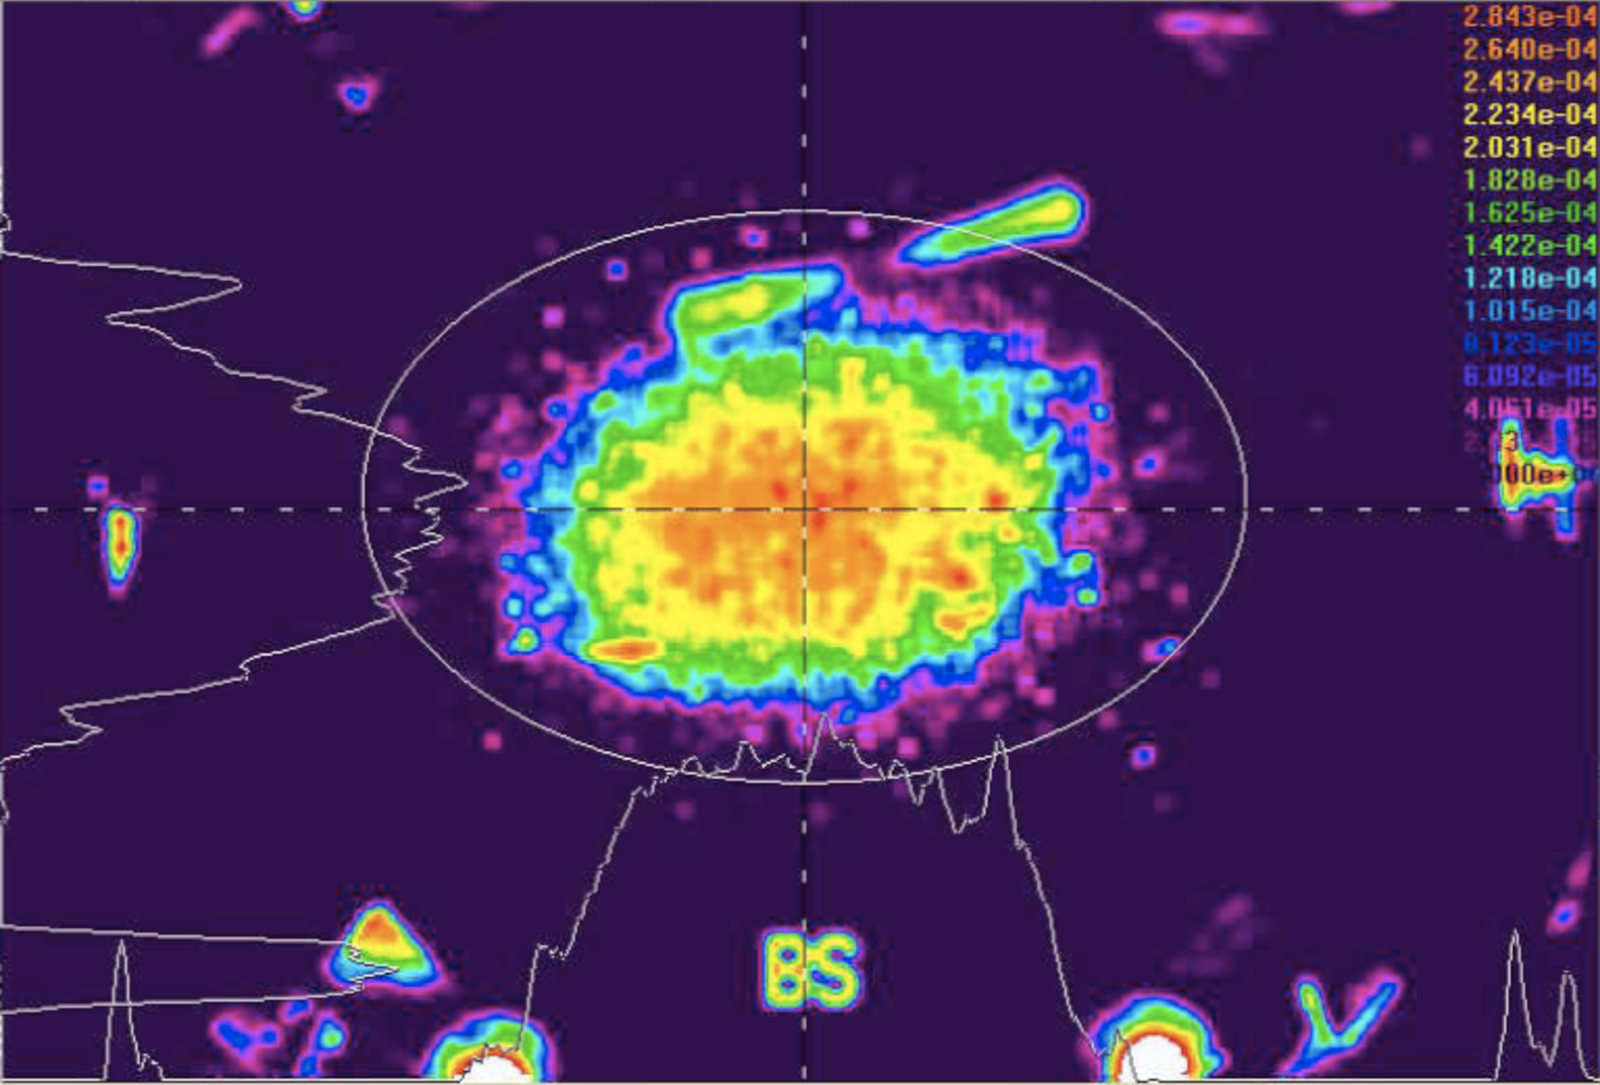
\includegraphics[width=0.6\textwidth]{figures/BCSspiricon.pdf} 
\caption[Beam centering servo image of beam splitter]{Image of beam on beam splitter as used in the beam centering servo. The beam appears stretched because the camera's viewing angle is at $45^{\circ}$ with respect to the mirror surface. The color scale is arbitrary.}
\label{fig:BCS}
\end{centering}
\end{figure}

The one additional step needed for full interferometer alignment is to maintain the orthogonality of the y-arm to the x-arm as the x-arm and input beam together move around. This is accomplished through the pitch and yaw signals of QPDY, the QPD that monitors the light transmitted through the y-arm, which sense how the beam splitter should be pointed. \footnote{QPDX also sends a signal to the BS to compensate for whatever it has MMT3 do.}

All mirror angles are of course interdependent and they must track each other. However, a rough hierarchy of who follows who can be established since ultimately the interferometer is bolted to the ground and necessarily maintains some DC orientation. This orientation comes from QPDX and QPDY, which are physically attached to piers standing on the ground and force the beams transmitted through the ETMs to stay put at a certain location on their sensors. In all, the input beam must make it to those two exact places and the other mirrors are left to line themselves up accordingly. A diagram of this alignment scheme is in Fig. \ref{fig:ASClayout}.

%two input beams, one to the x-arm, one to the y-arm; and the FPM

\begin{figure} \begin{centering} \includegraphics[width=0.8\textwidth]{figures/ASClayout_wctrl.pdf} 
\caption[Schematic of the alignment sensing and control system]{Schematic of the alignment sensing and control system, showing the placement of sensors and which mirrors they control. The QPD servo and Beam Centering Servo (BCS) together direct the input beam to follow the FPM unit on minute time scales. The QPD servo additionally keeps the BS properly directing light into the y-arm. The wavefront sensing servo maintains the alignment of the FPM mirrors with respect to each other up to several Hz. Each of the seven large optics has its own velocity damping optical lever servo.}
\label{fig:ASClayout}
\end{centering}
\end{figure}

This alignment process involving the WFS, QPDs, and BS camera relies on the entire interferometer already being locked. It manages the continuous fine-tuning of mirror angles so that maximal power buildup in the interferometer is maintained, and so that the interferometer does not wander from its linear operating point. How to achieve the initial alignment of all of the mirrors is an interesting process in itself and is documented in Appendix \ref{sec:initial_alignment}.


\section{Sources of mirror motion}
If the interferometer can be aligned well enough by hand for the initial lock to be achieved, one might wonder why the need for continuous tweaking thereafter. The answer is that there is a continuous stream of changing torque inputs to the mirrors that cause them to twist and turn in pitch and in yaw. Some torque inputs exist regardless of the state of the interferometer, while others are a direct consequence of the control systems. The primary torque inputs are introduced here, and further discussion of some of them is found later in the chapter. The list includes:
\begin{itemize}
\item ground motion \vspace{-10pt}
\item coil actuators (length to angle) \vspace{-10pt}
%\item thermal noise of pitch and yaw modes? \vspace{-10pt}
\item radiation pressure \vspace{-10pt}
\item noise impression from the angular control system 
\end{itemize}


\subsection{Ground motion} 
The most egregious of these torque inputs is ground motion that makes its way through the multiple stages of seismic isolation to the mirror suspensions. This is the only source of angular motion that is present regardless of the state of interferometer operation, and it is also AC damped at all times for each of the large optics through optical lever witnesses. Keeping the mirrors quiet enough with respect to their local ground is necessary to allow for the initial locking of the interferometer, so each suspended optic, small and large, is quieted by its OSEM signals during the initial locking stages. An example of the shape and amount of velocity-damped angular motion experienced by the core optics due to seismic noise during a relatively quiet seismic time is shown in Fig. \ref{fig:seismicMirror}. The rms mirror motion is of the order $10^{-7}$ rad. This is the motion that needs to be controlled interferometrically. 

\begin{figure}
\begin{centering}
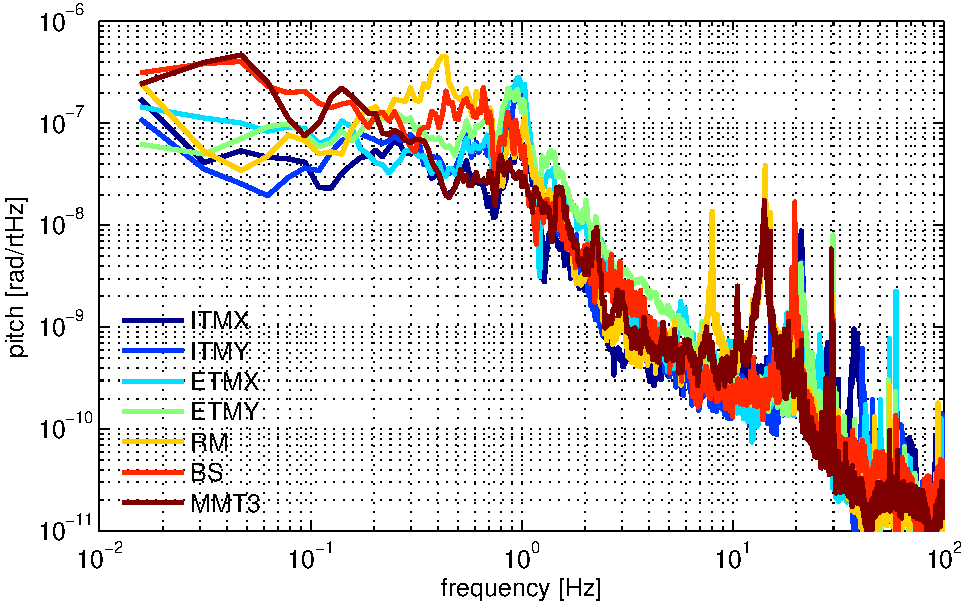
\includegraphics[width=1.0\columnwidth]{figures/seismic_mirrormotion.pdf}
%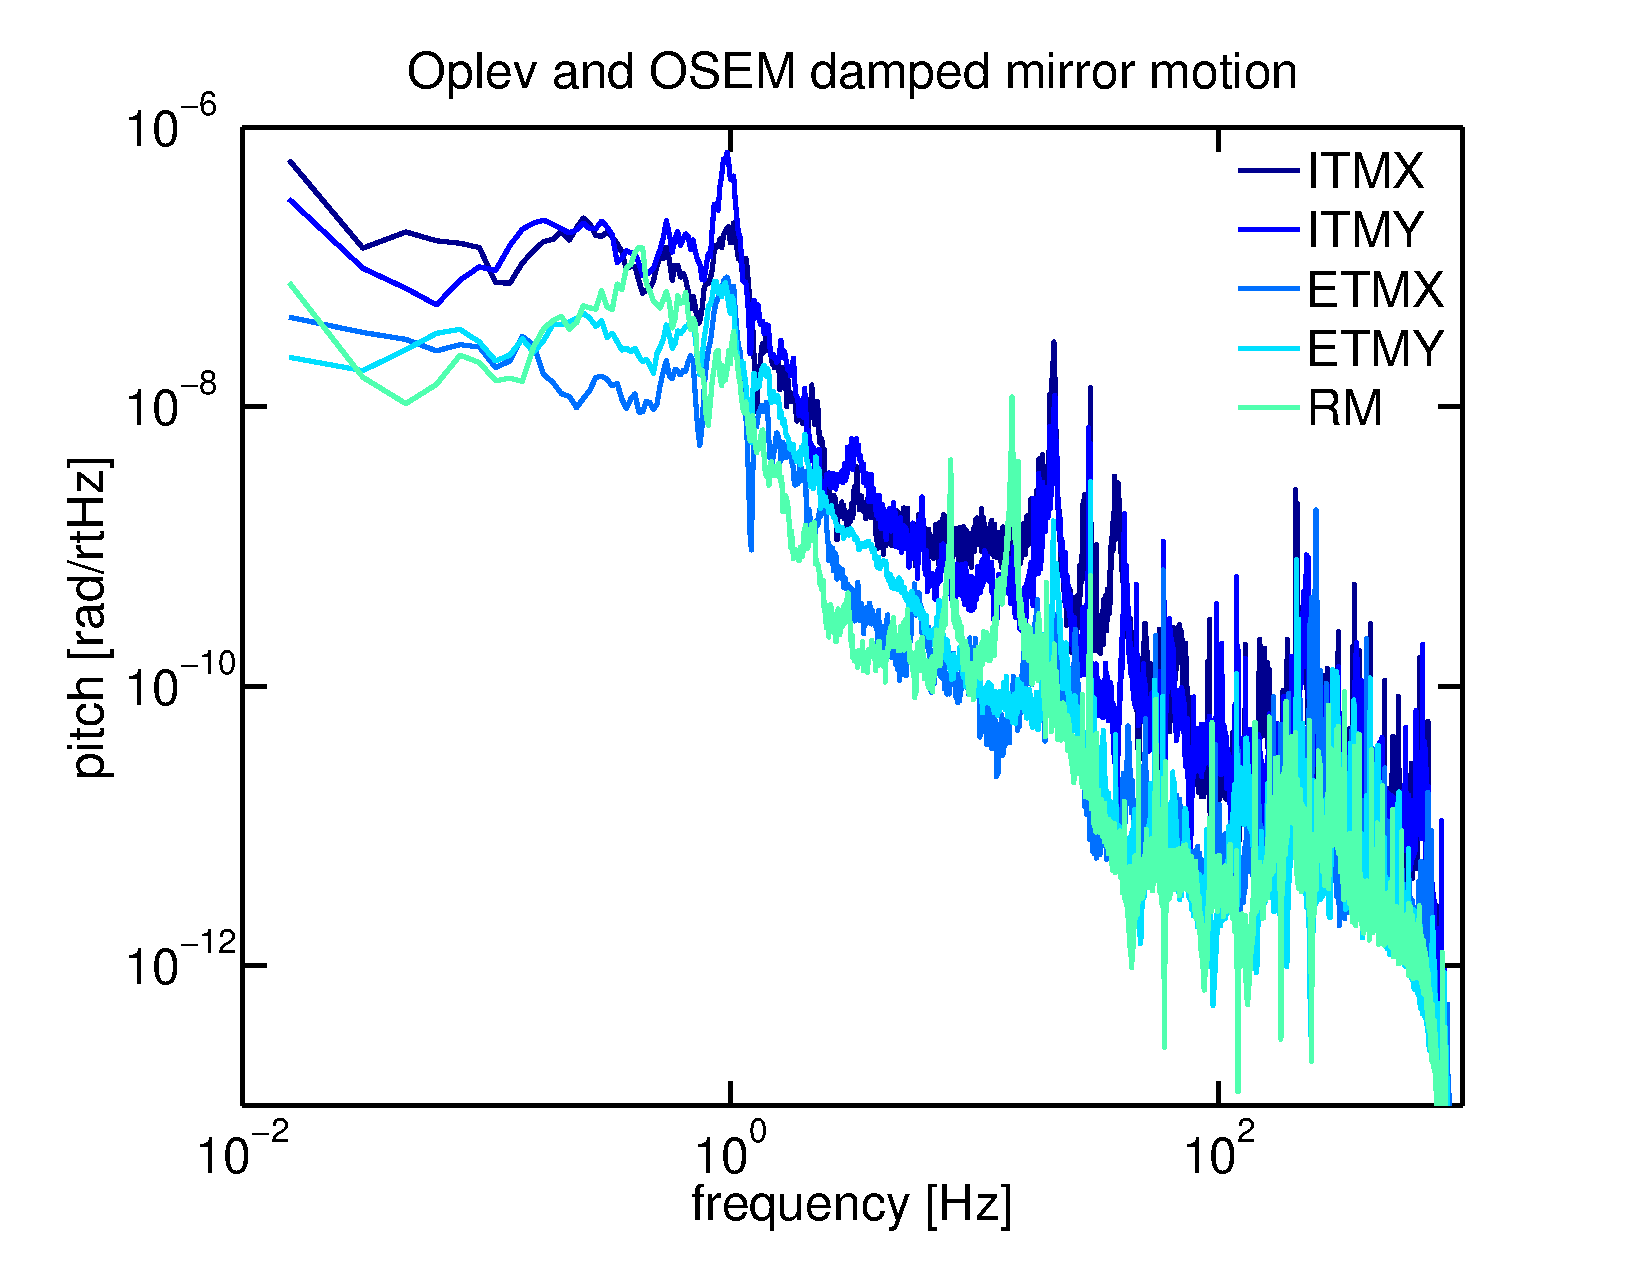
\includegraphics[width=0.7\columnwidth]{figures/ifodark_mirrormotion.pdf}
\caption[Typical angular motion of the core suspended mirrors in the
  absence of interferometric control]{Typical angular motion of the core suspended mirrors in the
  absence of interferometric control. Velocity damping provided by the
 OSEMs and the optical levers is present. Once the interferometer is locked, the OSEM damping is ramped off. 
  % Above about 30 Hz, the plot
  % does not represent real motion; the spectrum is limited by sensor
  % (optical lever) noise.
}
\label{fig:seismicMirror}
\end{centering}
\end{figure}

% Take a model of the optical lever open loop gains and a spectrum of
% optical lever error signal at a time when the interferometer is
% unlocked, but optical levers are on to calculate the background mirror
% motion due to seismic noise. Show the effect at a select few different
% times of day, probably for just one mirror. Write this section once I
% see what I have to present.





\subsection{Coil actuators} 
\label{sec:L2A}
The imperfect piston drive of the actuators on the rear of the test masses due to length control is another torque input, albeit inconsequential. The length of the cavities is carefully controlled (that's what we strive to be most sensitive to!) and any imbalances between the four electromagnets on a single mirror will create a coupling from length drive to angle (L2A). This effect is measurable, but is carefully tuned out through selecting appropriate digital gains for each of the coils. Typically, the gain variation from unity is up to 10\%. The residual is about 1\%. For the typical rms length drive of 1~\micron on a core optic and osems separated by a distance of $\sqrt{2} R$ where $R$ is the radius of the optic, the 1\% L2A coupling results in a $10^{-8}$ radian displacement:
\begin{equation}
\theta = \frac{0.01 * 10^{-6} \mbox{ m}}{\sqrt{2} * 0.125 \mbox{ m}} \approx 10^{-8} \mbox{ rad}.
\end{equation}

% Maybe include a figure that takes a typical length control spectrum signal to an optic and multiply by the above factors to show spectrum of angular motion induced by 1\% L2A.



\subsection{Radiation pressure} 
Radiation pressure creates a torque when the beam impinges the mirror
off-center. The force on the mirror due to radiation pressure is
derived from the change in momentum of a photon upon reflection off
the mirror and results in:
\begin{equation}
F_{rp} = \frac{2 P} {c}
\end{equation}
where $P$ is the power of the light reflected by the mirror and $c$ is the
speed of light. Assuming the beam of photons strikes the mirror
perpendicular to its surface, the torque exerted on a mirror due to
radiation pressure is
\begin{equation}
\tau_{rp} = \frac{2 P x} {c}
\label{eq:tau_rp}
\end{equation}
where $x$ is the distance of the beam from the mirror's center of mass. For a 40~kW beam 1~mm off-center, the torque is on the order of $10^{-7}$ Nm, corresponding to an angular displacement of the order $10^{-7}$ rad as determined by the pendulum torque to angle transfer function (see \ref{sec:pendTF}).

Amongst the various torque inputs, radiation pressure plays a unique role in mirror motion because the torque it exerts depends on the angles of the mirrors. This is a result of the geometric coupling between beam displacements and mirror angles as will be shown in the next chapter. Radiation pressure therefore acts as an angular spring. It is best treated not as an external torque, but as a modification to the pendulum torque to angle transfer function. Part of the next chapter dedicates a discussion to this matter. In all, radiation pressure shapes the angular dynamics of the mirrors in LIGO and plays an important role in the design of an angular control system.



\subsection{Noise from angular control}
The angular control system, which strives to counteract the above torque inputs to reduce angular motion, introduces angular mirror motion itself. The primary way it contributes noise is through imperfect sensing of the angular displacements. The control system also impresses input beam motion on the mirrors. These issues and others are explained in more detail in \ref{sec:ASClimits}.



\section{Tolerance for angular motion}
% Unlike DARM where the uncontrolled length displacement is what matters, it's the controlled  motion of the mirrors that matters for angular displacement. Too much residual motion, and both the lever arm effect and power fluctuations create noise in DARM. To prevent angular mirror motion from creating length displacements, the mirrors must not move more than $10^{-8}$ rad rms and the beam spots no more than 1 mm rms, as The residula motion must be held below 

The requirements for how much motion is tolerable stem from two effects of misalignment that directly couple to strain sensitivity: power build-up degradation, and angle to length coupling. The misalignment tolerances are dictated by what is necessary to prevent the strain sensitivity of the perfectly aligned interferometer from degrading by more than 0.5\% in the detection band of 40-7000~Hz \cite{Fritschel1997Alignment}.

Since the strain sensitivity is proportional to the power buildup (see Eq. \ref{}), a decrease in circulating power directly results in a decrease of shot-noise-limited DARM. Differing power fluctuations in the two arm cavities results in a changing contrast defect, a difference in the amount of light returning from one arm compared to the other, which increases the shot noise at the AS port. Too large of power fluctuations in the power recycling cavity makes for inconsistent signal to noise ratios for the signals that depend on sideband power. To maintain a power buildup within 1\% of maximum, the core optics must have an angular displacement of less than $10^{-8}$ rad rms with respect to the cavity axis \cite{ISCGroup1998ASC}. The derivation of power buildup as a function of mirror angle displacement is found in Appendix \ref{sec:cavitypower}.


\textcolor{blue}{work this paragraph in somewhere}
The idea is that when the axis of rotation of a mirror coincides with the center of the beam, any tilt of the mirror about this axis does not affect the path length of the reflected beam. However, if there is a mismatch between rotation axis and beam location, then the light will pick up a longitudinal phase shift when the mirror is tilted. During a full interferometer lock, this is recorded by DARM.



When the beam is located a distance $x$ away from the center of the mirror, an
angular displacement of the mirror $\theta$ about its center results in a path
length change of the beam
\begin{equation}
\Delta{L} = x * \theta
\end{equation}
which has a direct impact on DARM. Therefore, the alignment specifications must include not only tolerable levels of angular motion, but requirements for the physical centering of the beam spots on the mirrors. As detailed in Ref. \cite{ISCGroup1998ASC}, the beams must be centered on the core optics within 1~mm. At DC, for x ~=~1 mm and $\theta = 10^{-7}$ rad, $\Delta{L} = 10^{-10}$ m which is four orders of magnitude below the DARM rms of $10^{-6}$ m. \textcolor{blue}{Convolve my bsm spectra and residual mirror motion spectra to show example.}



\section{Angular control limitations}
\label{sec:ASClimits}
The limits for how good we can do in controlling the angular motion of the interferometer are governed by how well we are able to sense the angular motion. Several of the wavefront sensors' signals are dark-noise-limited above 20-25~Hz, as seen in Fig. \ref{fig:WFSdarknoise}. And depending on the power level, WFS1Q may instead be limited by shot noise (see Eq. \ref{eq:shotnoise}). Any control signal derived from frequencies in the sensing noise limited regime will impress the sensor noise on the mirrors. This cannot be avoided entirely in the presence of feedback, but can be mitigated by including amongst the control filters a steep cut-off beginning at the sensor noise frequencies. 
%Ultimately, it is the WFS noise floor that determines the best possible achievable suppression. 

\begin{figure} \begin{centering} \subfigure{\includegraphics[width=0.333\textwidth]{figures/wfs1q_darkres.pdf}}\subfigure{\includegraphics[width=0.333\textwidth]{figures/wfs2i_darkres.pdf}}\subfigure{\includegraphics[width=0.333\textwidth]{figures/wfs2q_darkres.pdf}} 
\subfigure{\includegraphics[width=0.333\textwidth]{figures/wfs3i_darkres.pdf}}\subfigure{\includegraphics[width=0.333\textwidth]{figures/wfs4i_darkres.pdf}} 
%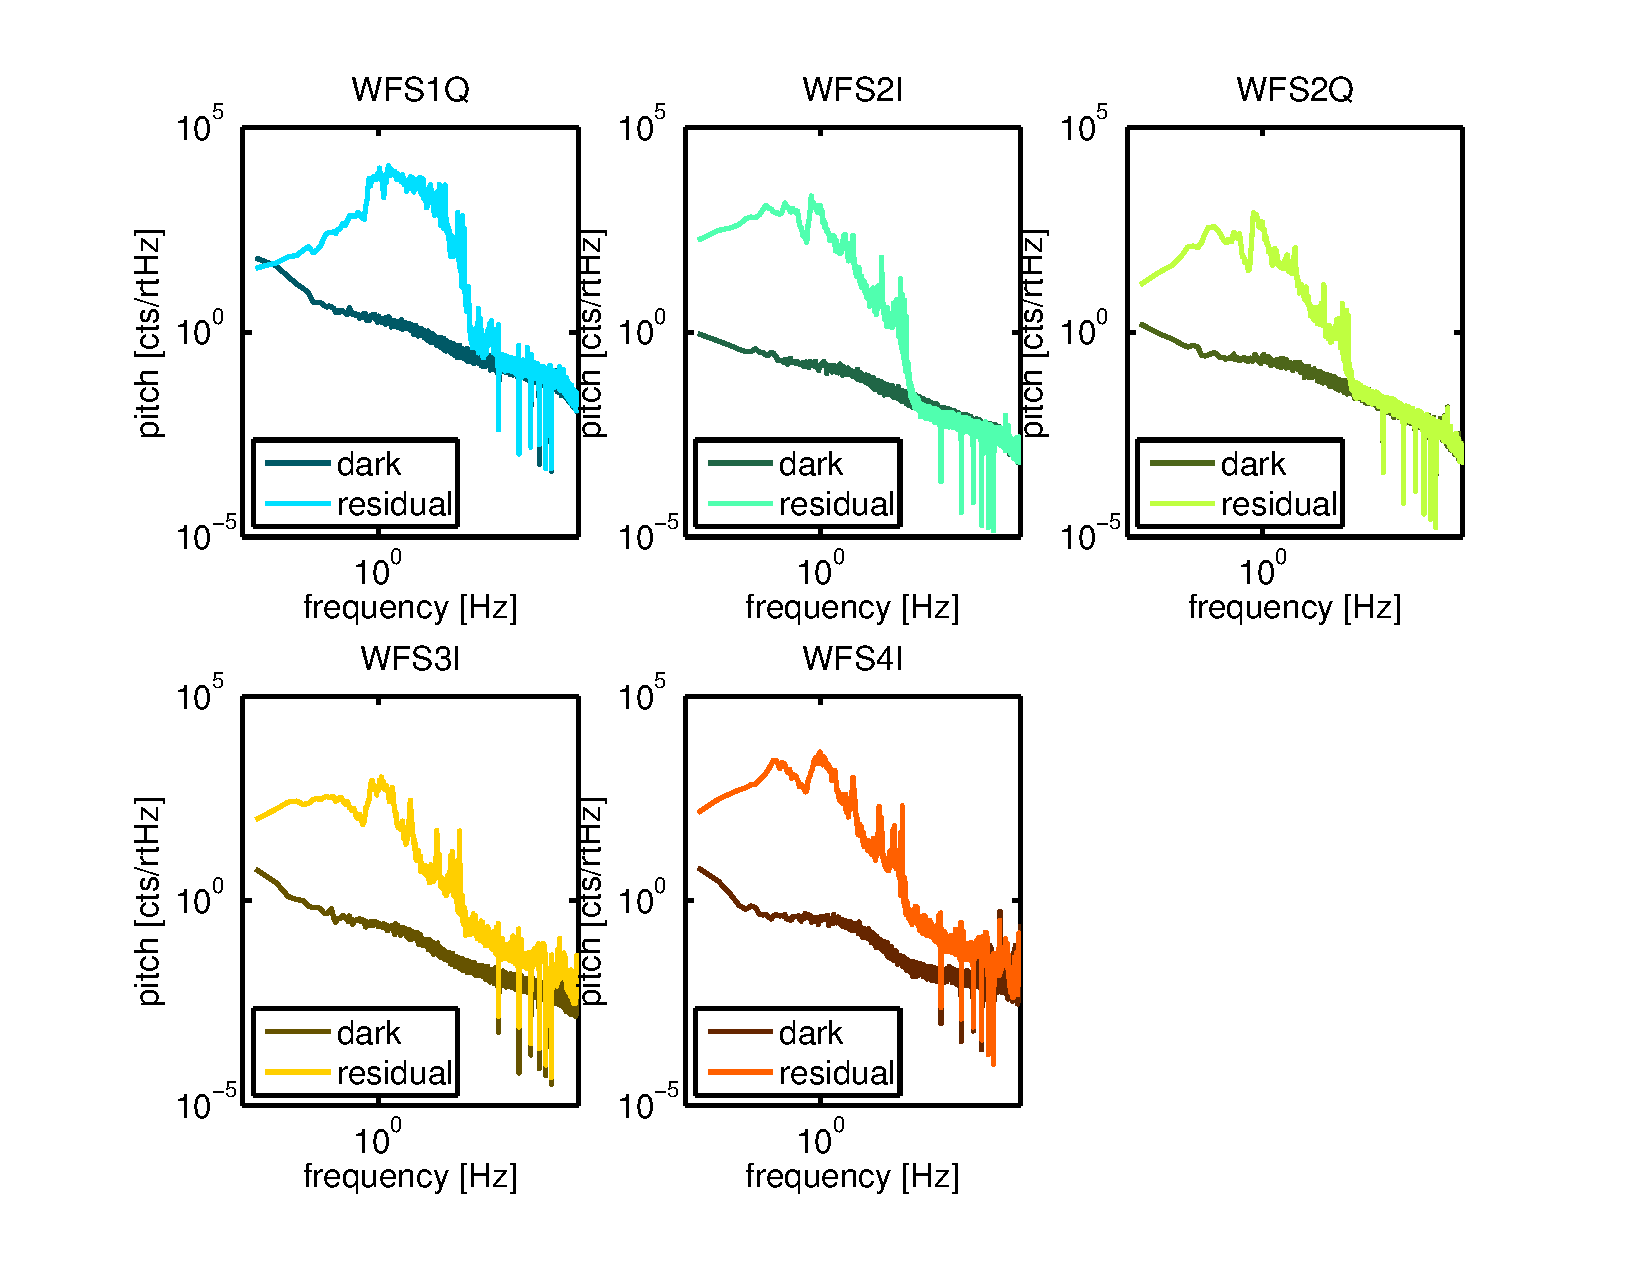
\includegraphics[width=1.0\textwidth]{figures/ASCsensorsignals.pdf} 
\caption[WFS error signal and dark noise]{WFS dark noise compared to typical error signal. \textcolor{blue}{Include shot noise, too, especially for WFS1.} The excess signal above the dark noise in WFS3I and WFS4I from 20~Hz on is likely acoustic noise, although this has not been verified. WFS1 and WFS2 are on a floating table in a sound proof chamber, while WFS3 and WFS4 are on a non-seismically isolated table without a sound proof enclosure.}
\label{fig:WFSdarknoise}
\end{centering}
\end{figure}

Besides the sensing noise, there is also sometimes real signal that results in more harm than good when used as feedback. The HAM seismic isolation tables used by the Input Optics (the core optics are suspended from BSC tables) have stack modes of xx Hz that ring up the MMTs.  At low frequencies, around 1~Hz, some of the WFS signals are dominated by these angular fluctuations of the input beam. The resulting attempt of the mirrors to follow the input beam jitter leads to a magnification of the motion because of the drastically different length scales. Large power fluctuations in both arms and the power recycling cavity ensue, leading to departure from the linear error signal regime and often lock loss. 

Other limitations to the reduction of mirror motion result from the nature of control loops. The cut-off filter, for example, reduces the phase margin of the open loop gain, necessarily pushing down the unity gain frequency (UGF) and therefore the magnitude of suppression at all frequencies below the UGF. A less aggressive cut-off filter, while improving the servo's stability and allowing for higher overall gains, leads to more impression of sensing noise on the optics. Also, when the phase margin of the loop is low, some mirror motion is amplified through gain peaking.

% A final point that should be noted, but is in fact insignificant, is a coupling from angular drive to length that results from the same principle of the length to angle coupling presented in \ref{sec:L2A}. 

% We will show that we don't quite meet all of these requirements and the impression of sensing noise in fact plays a major role in the reduction of DARM sensitivity up to 70 Hz.



\section{Wavefront sensing}
\label{sec:wfs}
Describe modes, reference sidebands, Gouy phases; give FP cavity example. 




